%%%%%%%%%%%%%%%%%%%%%%%%%%%%%%%%%%%%%%%%%%%%%%%%%%%%%%%%%%%%%%%%%%%%%%%%%%%%%%
%%
%% This file is part of the ASTERICS Framework. 
%%
%% Copyright (C) Hochschule Augsburg, University of Applied Sciences
%% Efficient Embedded Systems Group
%%
%% Author(s): Gundolf Kiefer <gundolf.kiefer@hs-augsburg.de>
%%
%%%%%%%%%%%%%%%%%%%%%%%%%%%%%%%%%%%%%%%%%%%%%%%%%%%%%%%%%%%%%%%%%%%%%%%%%%%%%%



\section{The Linux Kernel Driver} \label{ch:04-05-software-linux}

\secauthor{Alexander Zoellner}

\infobox{The Linux kernel driver is currently in development. The following text is in reference to an older version of the kernel driver - some information may be out of date.}

\subsection{Brief Description}

Within \asterics great emphasis is put on its usability for developing new image processing applications in a fast and convenient manner.
Utilizing an operating system is a common practice since it already provides a great deal of functionality, such as a network stack and memory management.
Further, required software is either already available or can be easily installed by using the package manager.
Being able to seamlessly integrate \asterics into own applications

As Linux is commonly used for embedded applications, the Linux character device driver \texttt{as\_driver} has been developed for \asterics.
This driver is able to operate with any \asterics-based image processing chain by providing a set of interfaces between hardware and software.
\asterics-chains can be exchanged on the FPGA without having to reload or recompile \texttt{as\_driver}.
The driver covers standard POSIX file operations, mapping memory regions to user as well as basic register-based hardware accesses.
The driver provides methods for altering the interfaces to hardware at runtime to cater to any \asterics-chain.


\subsection{Architecture}

Figure~\ref{fig:driver-architecture} shows the principle architecture of \texttt{as\_driver}.
It consists of the main parts \textit{device class}, \textit{device array}, \textit{file operation structures}, \textit{Init} and \textit{Exit}.
The latter two are methods which are the constructor and destructor of the kernel module, respectively.
They are called when the kernel module is loaded to the kernel or unloaded.
\textit{Init} performs the minimal required amount of initialization of the kernel module, such as registering it to the kernel and publishing its file operations.
For this reason, a \textit{device class} is created, which consists of a \textit{major number}, which refers to the kernel module itself and a number of \textit{minor numbers}.
Each \textit{minor number} is associated with a specific device of the kernel module, whereas the \textit{major number} indicates the responsible device driver for the device.
As shown in the figure, a number of \textit{minor numbers} are requested but not published immediately, indicated by \textit{empty} slots in the \textit{device class}.
The \asterics device driver organizes its devices in a \textit{device array} of a static size.
Devices may be added or removed from the \textit{device array}.
Slots which are not yet occupied by a device are indicated by \textit{uninitialized}.
Each device is associated with a \textit{minor number} and a \textit{file operation structure}.
The five \textit{file operation structures} are the actual device types available to \texttt{as\_driver}.
Each structure defines a set of \textit{methods}, which are used to overwrite the default file operation methods provided by the kernel.
This is accomplished by linking to one of these \textit{file operation structures} when initializing the device.
As shown by the \texttt{as\_memio} device, devices of the same type also point to the same \textit{file operations structure} and use its \textit{methods}.
The first device, namely the \texttt{as\_control} device, is created by \textit{Init} and the first \textit{minor number} is used.
Additional devices can be added or removed by using the \textit{methods} of the \texttt{as\_control} device, which publishes the device to the kernel by adding the associated \textit{minor number} to the \textit{device class} and linking to the appropriate \textit{file operation structure}.
\textit{Exit} on the other hand, deletes all allocated parts of the \asterics device driver and unregisters the kernel module and all its devices.
Resources obtained by the kernel module during its lifetime are released to the operating system again.

Up to this point, devices contained in the \textit{device array} are only known by the kernel but not yet accessible by the user application.
This requires to link the devices to the file system of the operating system in order to perform operations on the it.
A device can be published to the user space by creating a \textit{device node}, which is an entry point on the file system.
A \textit{device node} is associated with a certain device, by specifying its \textit{major} and \textit{minor number} upon creating the node.
As aforementioned, the \textit{major number} is used to tell the kernel which kernel module it should use when calling the file operations of the device.
The \textit{minor number} is used by the kernel module to identify the actual device to be accessed.
For creating the \textit{device node}, a path and a name on the file system has to be chosen where the node should appear.
When working with Linux, the location \textit{/dev/} is usually used for devices.
Once the \textit{device node} has been created, it can be used for the path argument for the open file operation to access the device and subsequently perform additional actions by calling the appropriate file operations.
Since the \textit{device node} is only a link to a device, it can also be created before the actual device exists, provided that the \textit{major} and \textit{minor number}, which is going to be used, is already known at this point.
Trying to access the \textit{device node}, without the actual device existing, will fail for obvious reasons.
The node can be used as soon as the associated device has been published to the kernel.
Naturally, if the device is removed, the node will cease to perform any accesses to the device.

The structure of \texttt{as\_driver} allows to create additional devices at runtime and therefore can be used for any \asterics-based image processing chain implemented on hardware.
Moreover, devices can also be deleted at runtime, with the kernel module displaying similar behavior as if it has just been loaded to the kernel.
Therefore, the processing chain can also be replaced at runtime, by simply instructing the kernel module to delete all devices and subsequently creating new ones.

\begin{figure}[ht]
    \centering
    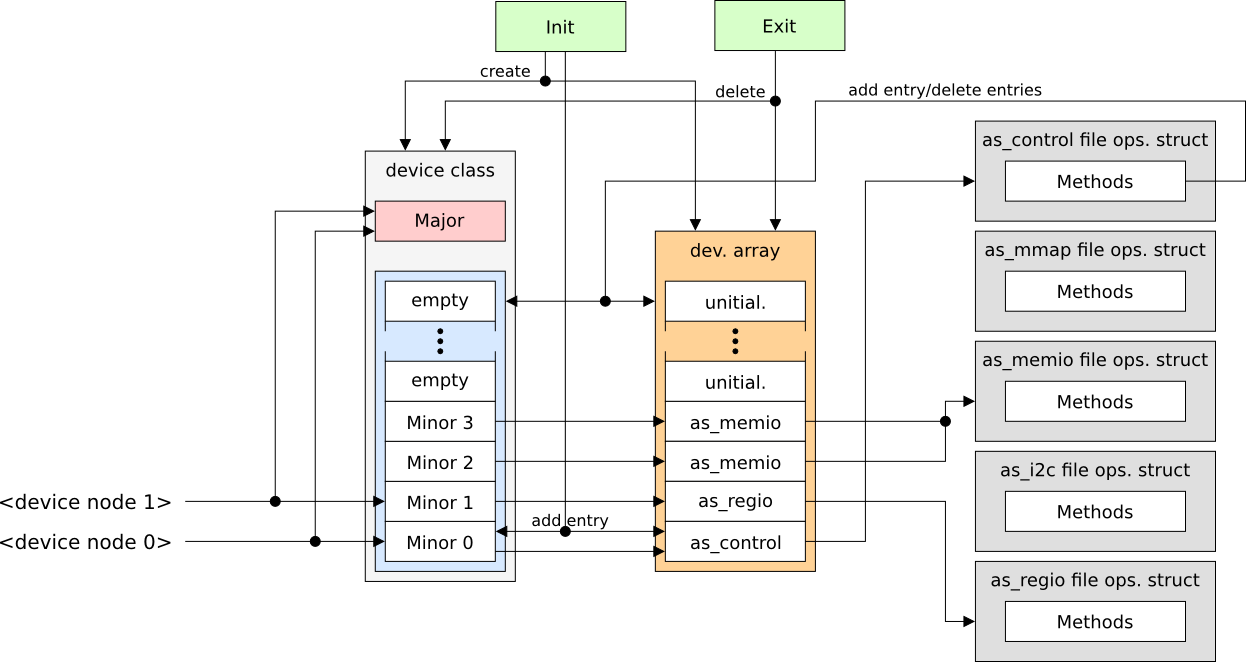
\includegraphics[width=0.8\linewidth,clip]{figs/driver_architecture.png}
    \caption{Architecture of the \asterics Linux kernel driver (\texttt{as\_driver})}
    \label{fig:driver-architecture}
\end{figure}

Table~\ref{table:device_driver:driver-files} lists the files of \texttt{as\_driver} and their meaning.
They can be found at "tools/as-linux/src/kernel\_module/asterics-driver".

\begin{longtable}[ht]{|l|c|l|l|}
    \hline
    \multicolumn{1}{|c|}{\textbf{Name}} & \multicolumn{1}{c|}{\textbf{Type}} & \multicolumn{1}{c|}{\textbf{Description}} \\
    \hline
    \texttt{as\_driver} & c source file & \parbox{7.5cm}{\ \\
        Implementation of the \asterics device driver.\\
    }\\
    \hline
    \texttt{as\_driver} & c header file & \parbox{7.5cm}{\ \\
        Compile time parameters and data structure of the \asterics device driver.\\
    }\\
    \hline
    \texttt{as\_linux\_kernel\_if} & c header file & \parbox{7.5cm}{\ \\
        Data structures and commands for \texttt{ioctl}/\texttt{unlocked\_ioctl} and device types used by the \texttt{as\_control} device. \\
    }\\
    \hline
    \texttt{as\_config} & c header file & \parbox{7.5cm}{\ \\
        Flags used for determining the features and environment the software has been compiled for. \\
        It is used for determining the appropriate implementation for functions provided by the \asterics software stack. \\
    }\\
    \hline
    \texttt{Makefile} & GNU makefile & \parbox{7.5cm}{\ \\
        Builds the kernel module.\\
    }\\
    \hline
    \caption{Files of the \asterics device driver}
    \label{table:device_driver:driver-files}
\end{longtable}


\subsection{Compile-Time Options}

The \texttt{as\_driver} offers a set of configuration parameters, which can be set at compile-time and therefore take effect, once the device driver is loaded.
Table~\ref{table:device_driver:config} lists the available parameters.
The device driver manages its devices in a list, with a fixed number of entries.
The parameter \texttt{NUM\_MAX\_DEVICES} is used to define the number of entries in the list, which correlates to the maximum number of devices which can be created by the \texttt{as\_control} device.
The number of devices has to be at least set to two, since one entry will be already occupied by the \texttt{as\_control} device.
As for the maximum number of entries, it is best to make use of the define found in the library \textit{kdev\_t.h}, which defines the maximum available amount of supported minor numbers for device drivers.
Each device requires a minor number in order for the kernel to distinguish between them.

The parameter \texttt{TIMER\_INTERVAL} is used to define the interval in jiffies for generating a timer interrupt.
The actual interval depends on the settings for \textit{HZ} of the platforms. 
For embedded platforms, it usually defaults to 100 Hz, which means the interval has a granularity of 10 ms.
Although the kernel provides an interface for converting a desired time in milliseconds to the appropriate number of jiffies, it cannot forgo the configured granularity of the interval.
This means, the resulting time may not match the actual requested time by the user, which could lead to confusion.
Thus, the parameter \texttt{TIMER\_INTERVAL} uses jiffies to clearly indicate its platform dependency.
An appropriate comment has also been added to the header file of the device driver to state this circumstance.
Depending on the expected amount of data to be transferred between software and hardware, this value can be increased or lowered accordingly.
For a low amount of data, the user may consider to increase the timer value, since calls to read or write of the \texttt{as\_memio} device may block for an extended period of time, until data becomes available again.
Since the interrupt is also used to wake up any sleeping processes, they might block immediately again, since no data has been become available between two consecutive interrupts.

\begin{longtable}[ht]{|l|c|c|l|}
    \hline
    \multicolumn{1}{|c|}{\textbf{Name}} & \multicolumn{1}{c|}{\textbf{Type}} & \multicolumn{1}{c|}{\textbf{Range}} & \multicolumn{1}{c|}{\textbf{Description}} \\
    \hline
    \texttt{NUM\_MAX\_DEVICES} & unsigned & 2 - MINORMASK & \parbox{5.5cm}{\ \\
        Maximum number of devices available to the driver \\
    }\\
    \hline
    \texttt{TIMER\_INTERVAL} & unsigned & 1 - 4294967295 & \parbox{5.5cm}{\ \\
        Timer interval in jiffies \\
    }\\
    \hline
    \caption{Configuration options for the ASTERICS device driver}
    \label{table:device_driver:config}
\end{longtable}


\subsection{Register-based IO Device}

In order to access the physical addresses of the hardware registers, they have to be mapped to a virtual kernel address area first.
Listing~\ref{code:regio-mapping} shows the functions, which have to be called for being able to access the physical address region.
The first function, \texttt{request\_mem\_region} is used to reserve a named address region from the kernel. 
By calling this function the driver tells the kernel, that it is going to use this address region.
No actual mapping is performed at this point, only a reservation request.
This prevents other drivers from mapping the same address region and thus competing accesses.
The first parameter \texttt{start} specifies the physical address, where the requested region starts, with a size of \texttt{n} bytes.
The last parameter \texttt{name} provides a pointer to a string, containing the name of the region.
If the request has failed, a NULL value is returned by these function, otherwise a non-NULL value.

The function \texttt{ioremap} is used to perform the actual mapping of the memory region.
It also requires the physical start address \texttt{start} of the region as well as its \texttt{size} in bytes.
The return value is a virtual kernel address, which can be used to perform the actual accesses to hardware.

The mapping of the memory region is performed by the \texttt{as\_control} device upon creating the \texttt{as\_regio} device.
Similarly, unmapping and releasing the memory region is either performed by the \texttt{as\_control} device or at the point \texttt{as\_driver} is unloaded.

\begin{lstlisting}[style=CStyle, label=code:regio-mapping, caption=Functions for allowing to access physical addresses]
struct resource * request_mem_region (
		unsigned long start, unsigned long n, const char *name)

void * 	ioremap (unsigned long phys_addr, unsigned long size)

\end{lstlisting}

The following Listing~\ref{code:regio-access} shows the functions used by the \texttt{as\_regio} device of the \asterics device driver for accessing the hardware registers of the hardware.
For obtaining the currently stored data in the hardware register, \texttt{ioread32} is used.
As the name suggests, it is used to read the value from the register at \texttt{addr}, which is the virtual kernel address, previously mapped by calling the aforementioned functions.
The return value is the current register content.
For writing data to the register, \texttt{iowrite} is used, which takes two parameters, the value to be written (\texttt{val}) and the virtual kernel address \texttt{addr}.
It is worth to note, that the currently used platforms, on which the device driver is used, are exclusively 32 bit systems and the hardware registers have also a size of 32 bits.

\begin{lstlisting}[style=CStyle, label=code:regio-access, caption=Functions for accessing hardware registers]
unsigned int ioread32(void __iomem *addr)

void iowrite32(u32 val, void __iomem *addr)

\end{lstlisting}

The \texttt{as\_regio} device provides only an implementation for the \textit{unlocked\_ioctl} method, whereas for open and close the default implementations provided by the kernel are used.
Similar to the \texttt{as\_control} device (Chapter TBD), the \texttt{cmd} parameter is used to inform the device, whether the method has been called by user or kernel space, in order to copy the data of \texttt{arg} appropriately.
The \texttt{unlocked\_ioctl} method can also be called by kernel space, since other devices of the \asterics device driver are also required to configure the hardware.
Instead of performing accesses to the hardware registers on their own, they make use of the \texttt{as\_regio} device.
The \texttt{arg} parameter of \texttt{unlocked\_ioctl} is a pointer to a \texttt{as\_ioctl\_params\_t} structure, which is part of \texttt{as\_linux\_kernel\_if.h}.
The \texttt{cmd} parameter of this structure can either be \texttt{AS\_IOCTL\_CMD\_READ} or \texttt{AS\_IOCTL\_CMD\_WRITE}.
In order to access the register correctly, the field \texttt{address} has to hold the physical address of the register.
This address may be obtained by the tools used for implementing the hardware design (e.g. Vivado).
For write accesses, the parameter \texttt{value} is written to the register, whereas for read accesses, the value of the register is directly returned by \textit{unlocked\_ioctl}, instead of copying it to the field of the structure.
The \texttt{user\_addr\_start} is not used by the \texttt{as\_regio} device and the user may decide to not explicitly assigning a value to it.

The user calls the associated \textit{ioctl} method with the same parameters.


\subsection{I2C Device}

The \textit{i2c device} works identically to the \texttt{as\_regio} device and uses the same kernel mechanisms for obtaining a memory region and accessing the hardware registers.
A separate device has been added to the \asterics device driver, to be able to map the hardware addresses of the used hardware registers to a different address region, which is not adjacent to the one used for the \texttt{as\_regio} device.
The actual functionality for the I2C uses the \texttt{as\_i2c} module driver, which utilizes the device driver for performing accesses to its hardware registers.


\subsection{Memory IO Device}

The \texttt{as\_memio} device utilizes the \texttt{as\_memio} module driver for conveniently transferring data between application software and FPGA.
For being able to transfer data, the \texttt{as\_memio} device has to be associated with a memory module, which in turn is forwarded to the \texttt{as\_memio} module driver.
In order to use a specific \texttt{as\_memio} device right away, this task is carried out upon creating the device with the \texttt{as\_control} device.
Here, the \textit{base address}, \textit{memory bus interface width} and \textit{direction} has to be provided.
The \textit{base address} is the address of the first hardware register used by the corresponding memory module, which is required for configuring the module correctly.
This address can usually be obtained by the tool used for implementing the processing chain on the FPGA (e.g. Vivado by Xilinx).

Similarly, the \textit{interface width} is needed for aligning the data correctly for its transfers. 
The memory modules are synthesized for a certain bit width, which is also used for its port towards other hardware modules.
For this reason, \emph{byte enables} are currently not supported, which results in having to transfer a multiple of the \textit{interface width} of bytes.

Since the \textit{direction} of the data flow is determined by either using an \texttt{as\_memreader} (to FPGA) or a an \texttt{as\_memwriter} (from FPGA) module, it has also to be provided to the \texttt{as\_memio} device.
Although the \texttt{as\_memio} module driver supports both directions, only one can be used at a time, since an instance of the driver only manages one memory module at a time.

The file operation structure for the \texttt{as\_memio} device provides implementations for five methods, namely \texttt{open}, \texttt{read}, \texttt{write}, \texttt{unlocked\_ioctl} and \texttt{close}.
Principally, the \texttt{open} method performs a number of checks and sets up the \texttt{as\_memio} module driver for the specific memory module.

In a first step, the \textit{device array} is iterated to find the \texttt{device\_data\_t} structure (part of \texttt{as\_driver.h}), which represents the requested \texttt{as\_memio} device. 
Multiple instances of the \texttt{as\_memio} module driver using the same memory module conflict with each other, due to relying on status information of the module regarding the current data transfer.
Therefore, only one instance of a given \texttt{as\_memio} device is allowed.
This is guaranteed by using the variable \texttt{busy} of the \texttt{device\_data\_t} structure, which is of type \textit{atomic\_t}.
Since the access to the variable is atomic, only one process can successfully acquire the \texttt{as\_memio} device.

After having acquired the corresponding \texttt{as\_memio} device, the directions \texttt{flags} provided upon \texttt{open} are compared to the one set at the point the device has been created.
In this way, the user is informed if the wrong device has been accidentally requested, e.g. data is to be transferred from memory to the FPGA but the device only supports inverse direction.
If this has been the case, the \texttt{as\_memio} device is released again and provides an error message to the user, pointing out this mismatch.

Otherwise, \texttt{as\_memio\_open} of the \texttt{as\_memio} module driver is called with a set of configuration parameters.
Except for the \textit{interface width}, the default settings defined in the header file of the \texttt{as\_memio} module driver are used.
The allocation of the \textit{Ring Buffer} and the \textit{Buffer Handler} is carried out by the module driver internally, without requiring the device driver to explicitly allocate structures on its own.
The module driver returns a pointer to the \texttt{struct as\_memio\_file\_s} structure, which is used by the module driver for managing the memory module.
The pointer is assigned to the \texttt{memio\_file} field of the \texttt{device\_data\_t} structure of the device.

As the \texttt{as\_memio} device supports blocking and nonblocking data transfers, the presence of the \texttt{O\_NONBLOCK} flag is checked.
If this flag has not been provided upon calling \texttt{open}, a \textit{wait queue} is set up for the device, allowing it to sleep if the request number of bytes cannot be served right away.
Lastly, the variable \texttt{memio\_active} is set to inform the interrupt logic to serve this device.
Figure~\ref{fig:memio-open} summarizes the steps performed by the \textit{open} file operation method.

\begin{figure}[ht]
    \centering
    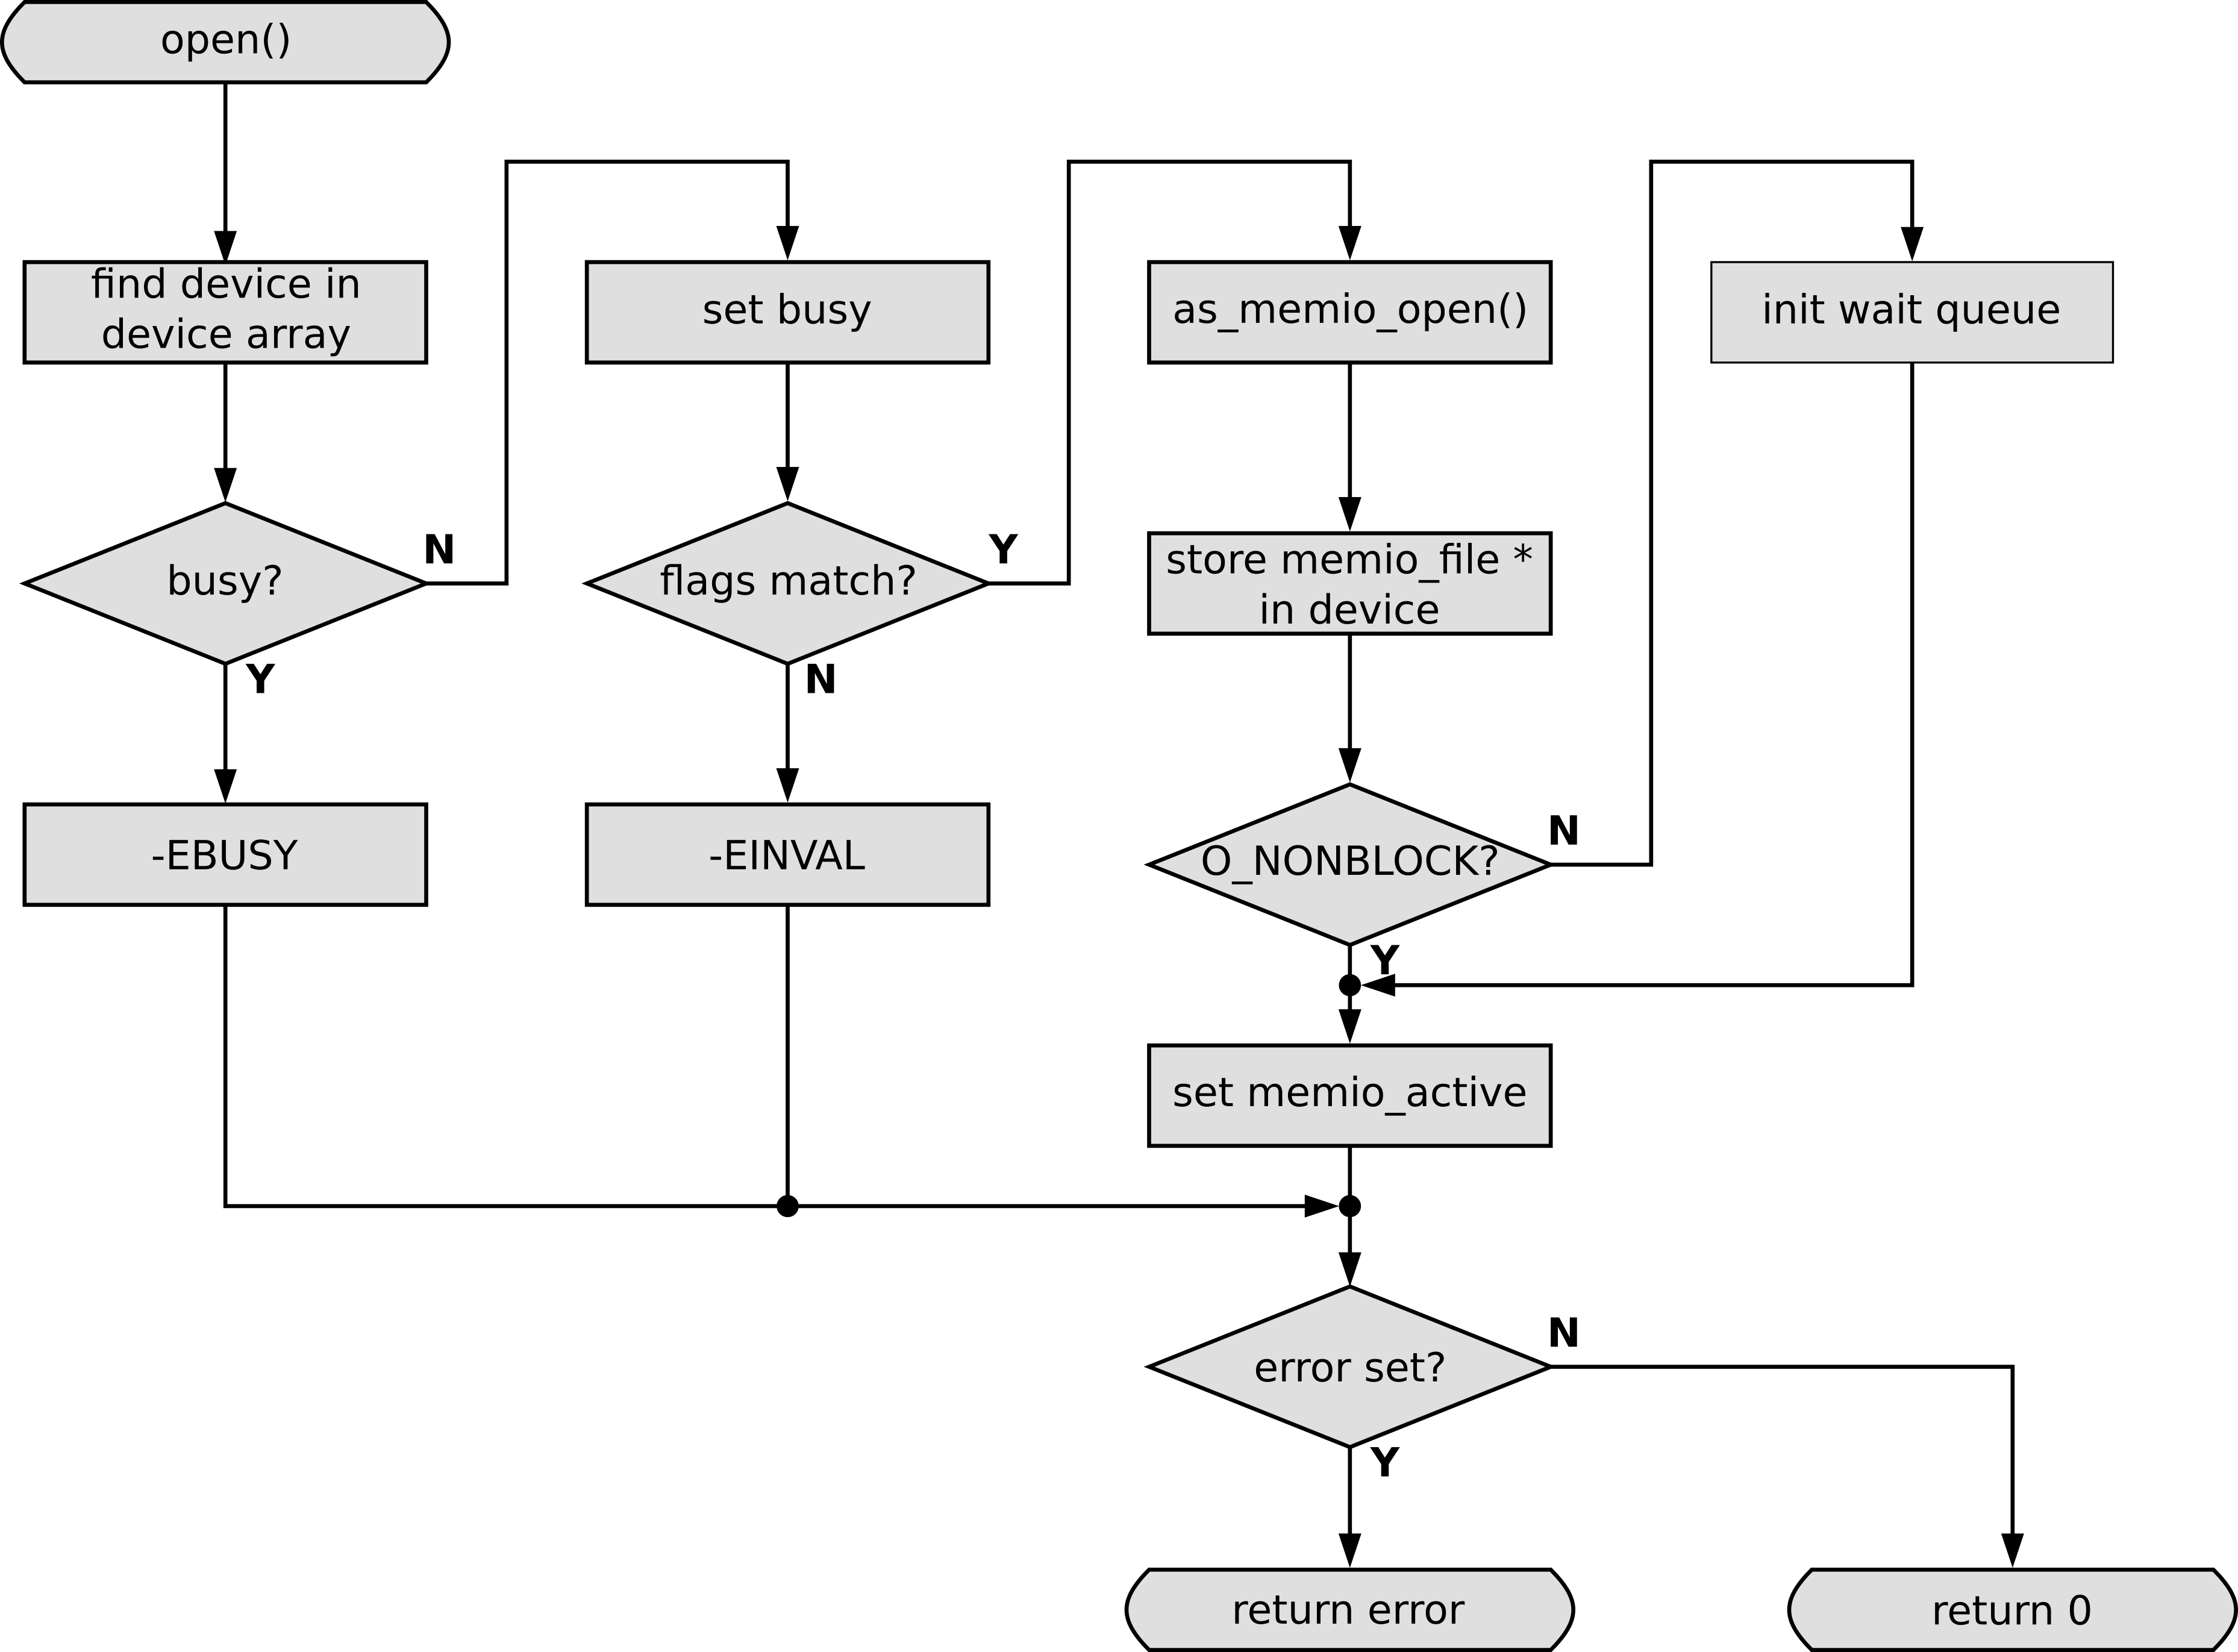
\includegraphics[width=0.7\textwidth,height=0.7\textheight,keepaspectratio]{figs/memio_open.png}
    \caption{Processing steps performed by the \texttt{open} method of the \texttt{as\_memio} device.}
    \label{fig:memio-open}
\end{figure}

For actually transferring data between main memory and the FPGA, the methods \texttt{read} and \texttt{write} are used.
In order to prevent race conditions of multiple processes trying to read or write data at a given time, using the same \texttt{as\_memio} device, a \textit{mutex} is used.
For this purpose, the \texttt{device\_data\_t} structure of the device provides the variable \texttt{access\_lock}.
Similar to \texttt{open}, the provided direction flag is evaluated, since only either of the two file operations is supported, depending whether a \texttt{as\_memreader} or \texttt{as\_memwriter} module is associated.
If the requested file operation is not supported by the specific \texttt{as\_memio} device, an error message points out the mismatch and a negative value is returned.
For this reason, the user has to evaluate the return value of the used function, at least for the first call.

Subsequently, the presence of \texttt{O\_NONBLOCK} is checked.
If the flag has been provided, the specified number of bytes and the \textit{User Buffer} is passed to the \texttt{as\_memio\_[read/write]} function of the \texttt{as\_memio} module driver.
The \textit{Buffer Handler} tries to serve the request as far as possible by transferring data between the \textit{User Buffer} and the \textit{Ring Buffer} and configuring the associated memory module accordingly.
Since the data cannot be directly copied between user and kernel space, the function  \textit{copy\_[to/from]\_user} has to be used.
Therefore, the module driver checks whether it has been compiled for the Linux kernel or for a bare-metal application, using the setting provided by \texttt{as\_config.h}.
The actually transferred number of bytes is returned to the \texttt{as\_memio} device, which is equal or less than the requested number of bytes.
This number is then passed to the user, returning immediately without blocking even if the requested number has not been met.
The POSIX standard states, that a negative return value shall be passed to the user, in case no data has been transferred at all and the device would block with the \texttt{O\_NONBLOCK} flag being set.
However, since the \texttt{as\_memio} device does not block under any circumstance if the \texttt{O\_NONBLOCK} flag has been provided, no error code is returned in this case.
The \texttt{read/write} functions simply returns with a "0" for the number of bytes, which have been transferred.
The caller of the corresponding function is expected to evaluate the return value and call the function again, if the requested amount has not been served entirely.

If the \texttt{O\_NONBLOCK} flag is absent, the \texttt{as\_memio} device performs the same call to the \texttt{as\_memio} module driver.
If the module driver has been able to perform the data transfer completely, the method behaves in the same manner as if the flag had been provided.
However, in case the transferred number of bytes is less than specified, the \texttt{as\_memio} device sets up the condition variable \texttt{wake\_up\_cond} and sets the flag \texttt{register\_intr} before blocking by calling the function \texttt{wait\_event\_interruptible}.
The processor stops executing the blocking process.
When the interrupt handler wakes up the process again by setting the condition variable appropriately and calling the function \texttt{wake\_up\_interruptible}, the device driver calls \texttt{as\_memio\_[read/write]} function again with the remaining bytes to be transferred.
If the request has been served entirely, the file operation method of the \texttt{as\_memio} device exits.
Otherwise, the above mentioned procedure is repeated.
When exiting, the mutex is released again.
Figure~\ref{fig:memio-transfer} summarizes the processing steps performed by the \texttt{read} and \texttt{write} method of the \texttt{as\_memio} device.

\begin{figure}[ht]
    \centering
    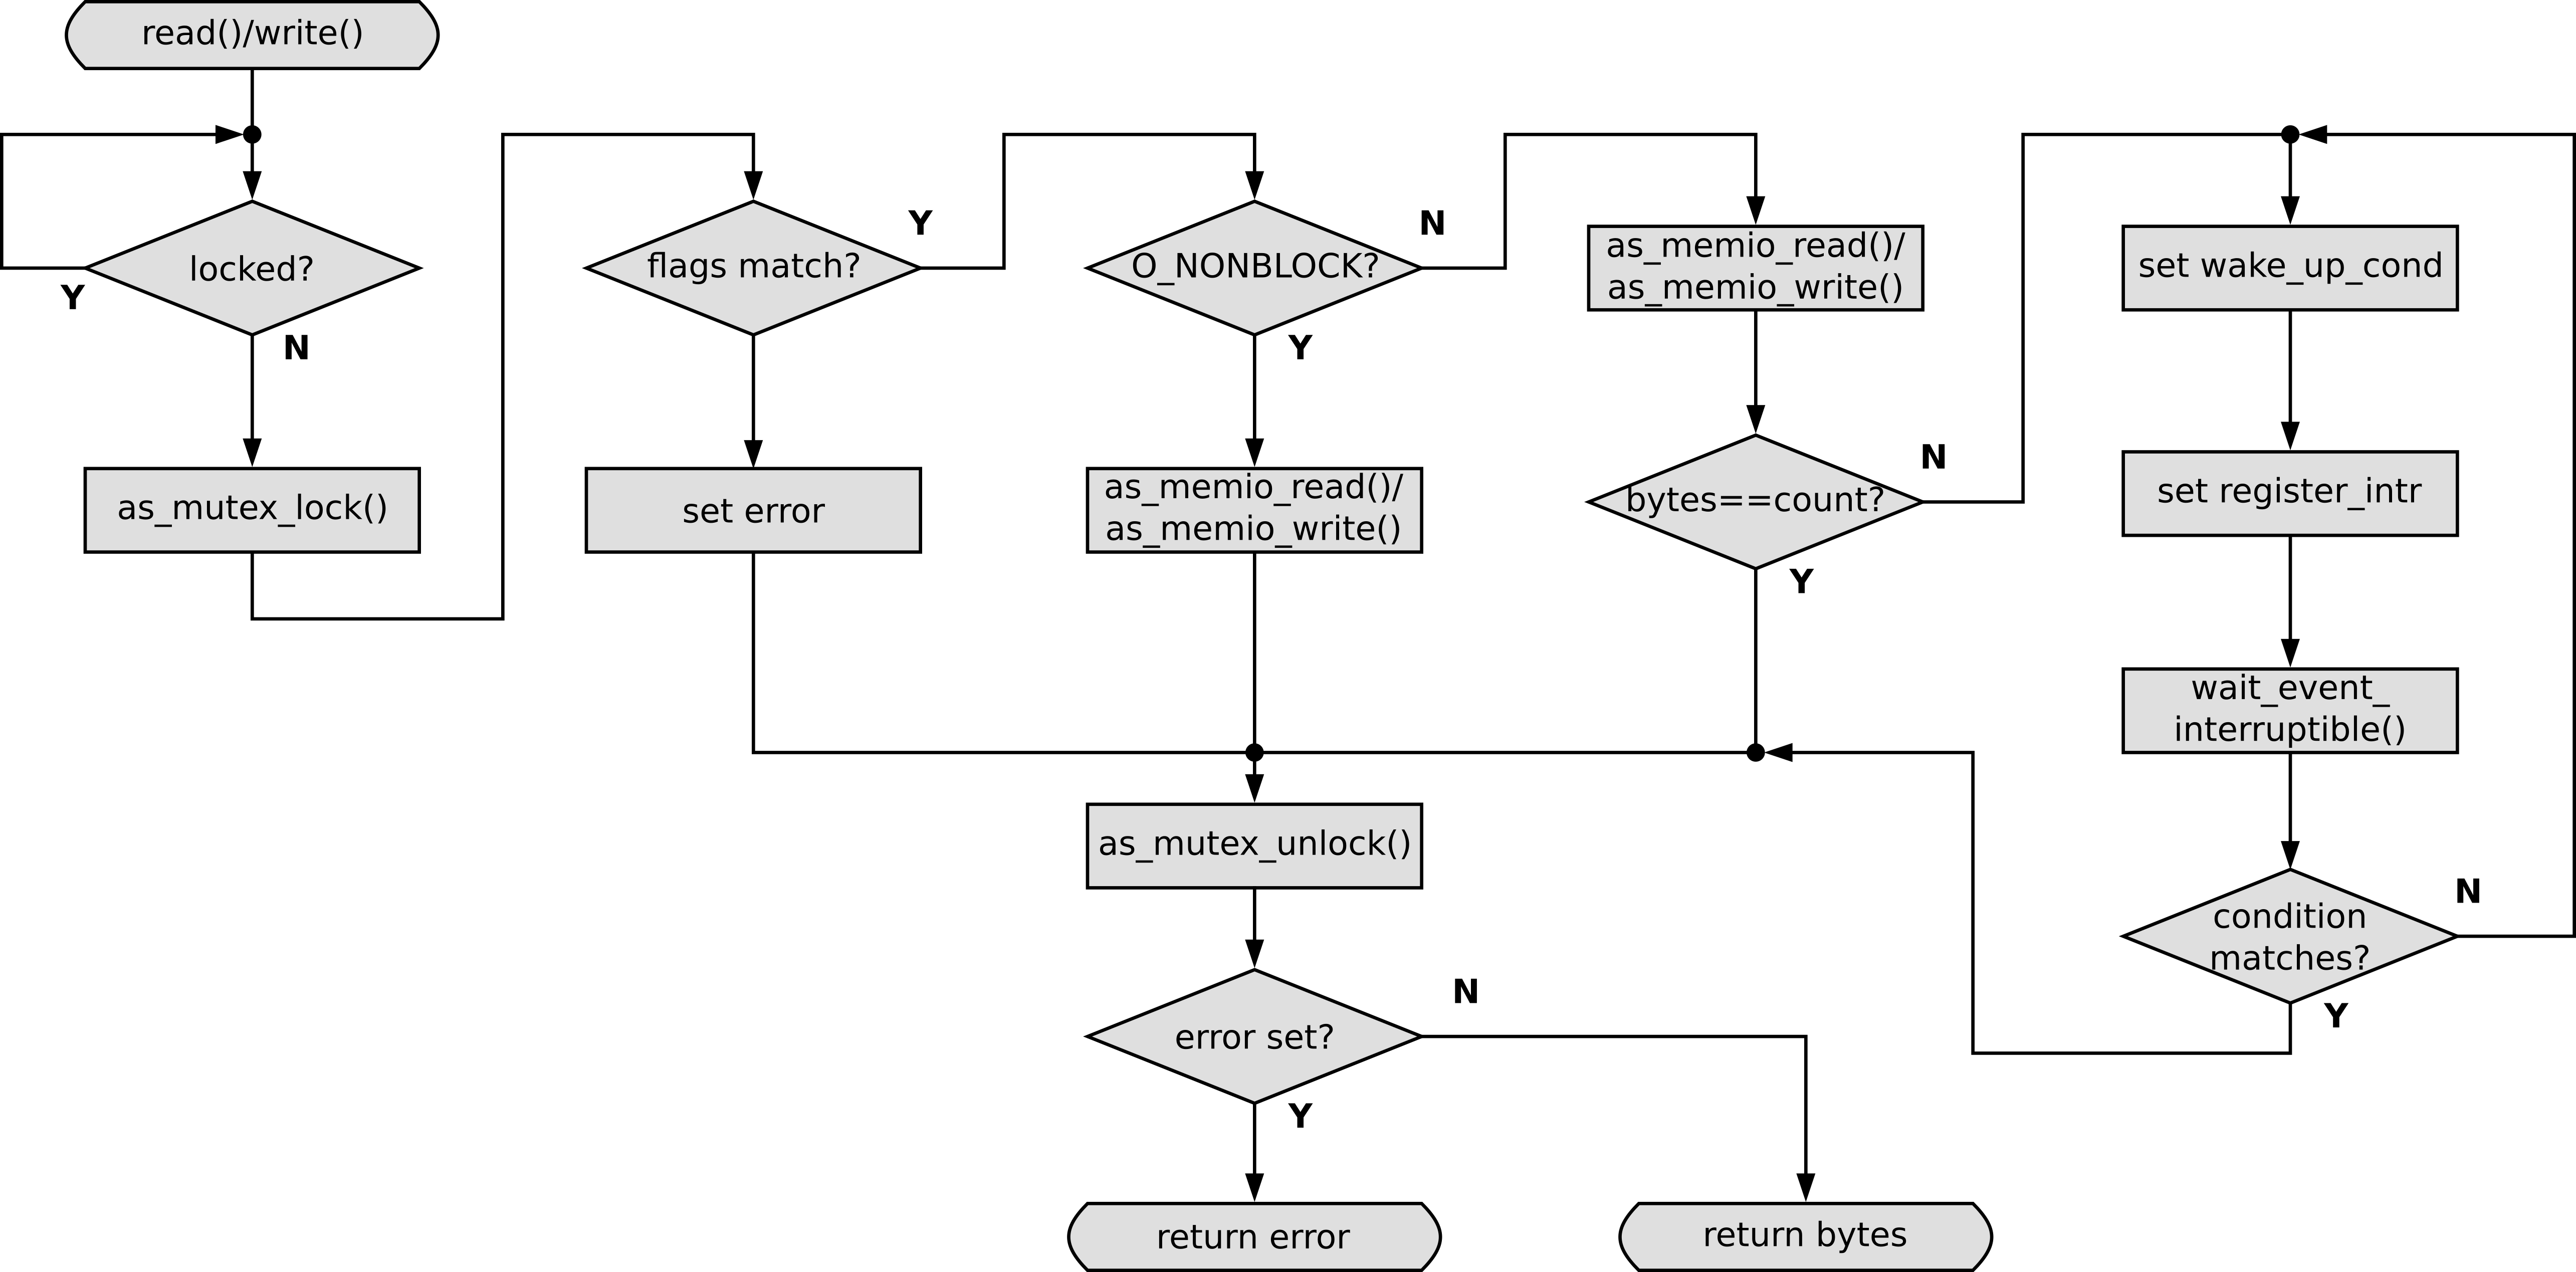
\includegraphics[width=\textwidth,height=\textheight,keepaspectratio]{figs/memio_transfer.png}
    \caption{Processing steps performed by the \textit{read} and \textit{write} method of the \texttt{as\_memio} device.}
    \label{fig:memio-transfer}
\end{figure}

The \texttt{unlocked\_control} method of the \texttt{as\_memio} device is used to trigger the \textit{Buffer Handler} of the \texttt{as\_memio} module driver to check whether there is data within its \textit{Ring Buffer} to be transferred.
The \texttt{as\_memio\_hw\_update} function of the module driver is used, by providing the pointer to the \texttt{memio\_file}.
Although this function is called by the module driver for every read and write request, it may occur that two calls to this function are required for transferring all data.
This is caused by the discrepancy of the differing access types of the \textit{Buffer Handler} and memory module to the \textit{Ring Buffer}.
The former writes or reads circularly to or from the \textit{Ring Buffer}, i.e. if the upper boundary is reached, it continuous at the lower boundary automatically.
The memory module, however, can only perform data transfers on physically concurrent memory addresses.
If a wrap around is required, the \textit{section} of the memory module has to be configured up to the upper boundary of the \textit{Ring Buffer} and the second one starting at the lower boundary again.
Usually, an explicit call to the \texttt{unlocked\_ioctl} method is not required, since the interrupt handler of the \asterics device driver regularly calls \texttt{as\_memio\_hw\_update} for its \texttt{as\_memio} devices, which are currently being used (see Chapter~\ref{device_driver:interrupts}).\newline

The \texttt{close} method of the \texttt{as\_memio} device resets the two variables, which are used for the interrupt logic of the device driver, \texttt{memio\_active} and \texttt{register\_intr}. 
In order to return the acquired resources by the \texttt{as\_memio} module driver back to the kernel, it calls the function \texttt{as\_memio\_close}.
Additionally, the module driver performs a reset on the associated memory module.
This terminates all ongoing data transfers, since the allocated \textit{Ring Buffer} is deleted and thus the memory area is no longer valid.
The \texttt{as\_memwriter} assumes a passive behavior, which prevents it from blocking any associated hardware processing chain.


\subsection{Memory Mapped IO Device}

The \texttt{as\_mmap} device circumvents having to copy data on memory by utilizing a dedicated memory area, which is published to the user. 
This memory can be shared between hardware and software.
Since the Linux operating system utilizes virtual address spaces, actual physical memory cannot be accessed from user space in the same way as its virtual addresses.
However, this limitation can be lifted to some degree, by utilizing mechanisms provided by the kernel to publish certain areas of physical memory to the user.
This is accomplished by implementing the file operation method \texttt{mmap} in a device driver for mapping a physically concurrent area of memory into the virtual address space of the user.
For this reason, the \texttt{as\_mmap} device has to provide a memory area which meets the requirements for being able to be mapped.
Regarding the lifetime of a device driver, the required memory can be acquired at several stages, such as at the time being loaded as kernel module, upon device creation or when the corresponding device is actually used.
Since \texttt{as\_driver} aims at being operable for any kind of image processing chain without having to reload the kernel module, the actual number of devices required by the user cannot be determined at the time it is being loaded to the kernel.
As the aforementioned memory areas are only utilized by devices of the \texttt{as\_mmap} type, a single memory area is allocated for each \texttt{as\_mmap} device upon creation, using the \texttt{as\_control} device.
The size of the memory area is configurable by providing the appropriate parameter to the \texttt{as\_control} device.
The memory area is acquired by using the kernel function \texttt{\_\_get\_free\_pages}, which allocates a physically concurrent amount of memory and returns the start address of it, i.e. a virtual kernel address.
This address is stored within the device to be used later on for the file operation methods.
As a side note, only sizes up to 4 MB have been used.
Allocations are to the power of two.
For preventing memory leaks, the memory has to be released when the corresponding device is no longer needed, i.e. when it is deleted.

As already stated, it would also be possible to allocate the memory when using a file operation method, such as \texttt{open}.
However, allocating memory can take quite some time, especially when trying to acquire larger areas of memory.
Additionally, it tends to get worse the longer the system runs, as memory gets fragmented.
Usually, when the user attempts to interacts with a certain device, the associated functionality is to be utilized immediately without further downtime.
For this reason, the memory allocation has been shifted to the point, where the device is created, i.e. the \texttt{as\_control} device.

Once \texttt{open} has been called on the device, the allocated memory region can be mapped using the file operation \texttt{mmap}.
For the \texttt{open} and \texttt{close} file operations, the default implementations provided by the kernel are used.
For actually mapping the allocated memory to the user space, the \texttt{vm\_end} and \texttt{vm\_start} field of the provided \textit{virtual memory aread (vma)} structure for \texttt{mmap} is used.
The difference between both is used for determining the number of bytes to be mapped.
If the number of bytes is equal or less than the one of the allocated area, the requested amount is mapped into the virtual address space of the user.
Listing~\ref{code:regio-mapping} lists the functions used for the actual mapping.
The first one, \texttt{virt\_to\_pfn}, is a macro for determining the \textit{page frame number (pfn)} of a given virtual address.
Since \texttt{\_\_get\_free\_pages} returns a virtual kernel address for the allocated memory area, this address is used.
The page frame number is required by the following function \texttt{remap\_pfn\_range}, which performs the actual mapping.
For the argument \texttt{virt\_addr}, the \texttt{vm\_start} field of the \texttt{vma} structure is used and for \texttt{size} the aforementioned difference of the \texttt{vm\_end} and \texttt{vm\_start} field.
Similar, the \texttt{vm\_page\_prot} field is used for the \texttt{prot} argument.
Usually, the user has to provide \texttt{PROT\_READ} and \texttt{PROT\_WRITE} when calling \texttt{mmap} from user space in order to be allowed to read and write to the mapped region.
The kernel provides the virtual address to user after the mapping, without requiring the developer of the device driver to perform any additional tasks.

\begin{lstlisting}[style=CStyle, label=code:regio-mapping, caption=Functions for allowing to access physical addresses]
#define virt_to_pfn(kaddr)

int remap_pfn_range(struct vm_area_struct *vma, unsigned long virt_addr,
				unsigned long pfn, unsigned long size, pgprot_t prot);

\end{lstlisting}

% unlocked\_ioctl
% - search mmap device
% - check if provided address is within mapped area 
Although the user can perform read and write accesses to the mapped memory area, transferring data to or from the hardware requires an explicit configuration of an appropriate memory module, depending on the desired direction.
This task is accomplished by using the file operation \texttt{ioctl} in user space, which results in calling the \texttt{unlocked\_ioctl} method of the \texttt{as\_mmap} device by the kernel.
For its \texttt{arg} parameter, the \texttt{as\_ioctl\_params\_t} structure is used.
The \texttt{cmd} field is used for determining the direction of the transfer, which can either be \texttt{AS\_IOCTL\_CMD\_READ} or \texttt{AS\_IOCTL\_CMD\_WRITE}.
The commands are defined in the interface header file \texttt{as\_linux\_kernel\_if.h} of the device driver.
The former requires a \texttt{as\_memwriter} module, whereas the latter requires a \texttt{as\_memreader} module.

The following parameter \texttt{address} specifies the base address of the memory module to be used for the data transfer.
Since the \texttt{as\_mmap} device is not bound to a specific memory module, an appropriate memory module has to be associated, which is either a \texttt{as\_memreader}, if the parameter \texttt{AS\_IOCTL\_CMD\_WRITE} has been provided, or a \texttt{as\_memwriter} for \texttt{AS\_IOCTL\_CMD\_READ}.
In order to find an appropriate memory module, the \textit{device array} is iterated to check if a \texttt{as\_memio} device exists, which is associated with the desired memory module.
This way, the \texttt{as\_mmap} device can use any of the defined memory modules within \texttt{as\_driver}.
If the memory module is defined within a \texttt{as\_memio} device, it checks the \texttt{busy} flag of the device, whether it is currently in use, i.e. the file operation \texttt{open} has been called on the requested \texttt{as\_memio} device.
By checking the flag, the device driver prevents interfering with any ongoing data transfers or the \textit{Buffer Handler}.
The flag is a variable of the type \textit{atomic\_t} which also helps to prevent possible race conditions for acquiring the shared resource, i.e. the memory module.

The \texttt{value} parameter is used to specify the number of bytes to be transferred between hardware and software.
Here, the device driver checks whether the requested amount can be transferred with the memory bus interface width used by the memory module.
The number of bytes has to be a multiple of the interface width.
Otherwise, a message is printed by the device driver to indicate the mismatch.

Lastly, the parameter \texttt{user\_addr\_start} is used to choose the start address within the memory mapped area, where the data transfer is supposed to begin.
The address is desired starting point within the virtual address space mapped to the user and is translated into the associated physical memory address.
Figure~\ref{fig:ioctl_mapping} illustrates the combination of the \texttt{user\_addr\_start} and \texttt{value} parameter for determining the memory area to be used for the data transfer.
The sum of both parameters must not exceed the boundaries of the memory area, as the device driver will perform any data transfer.

\begin{figure}[ht]
    \centering
    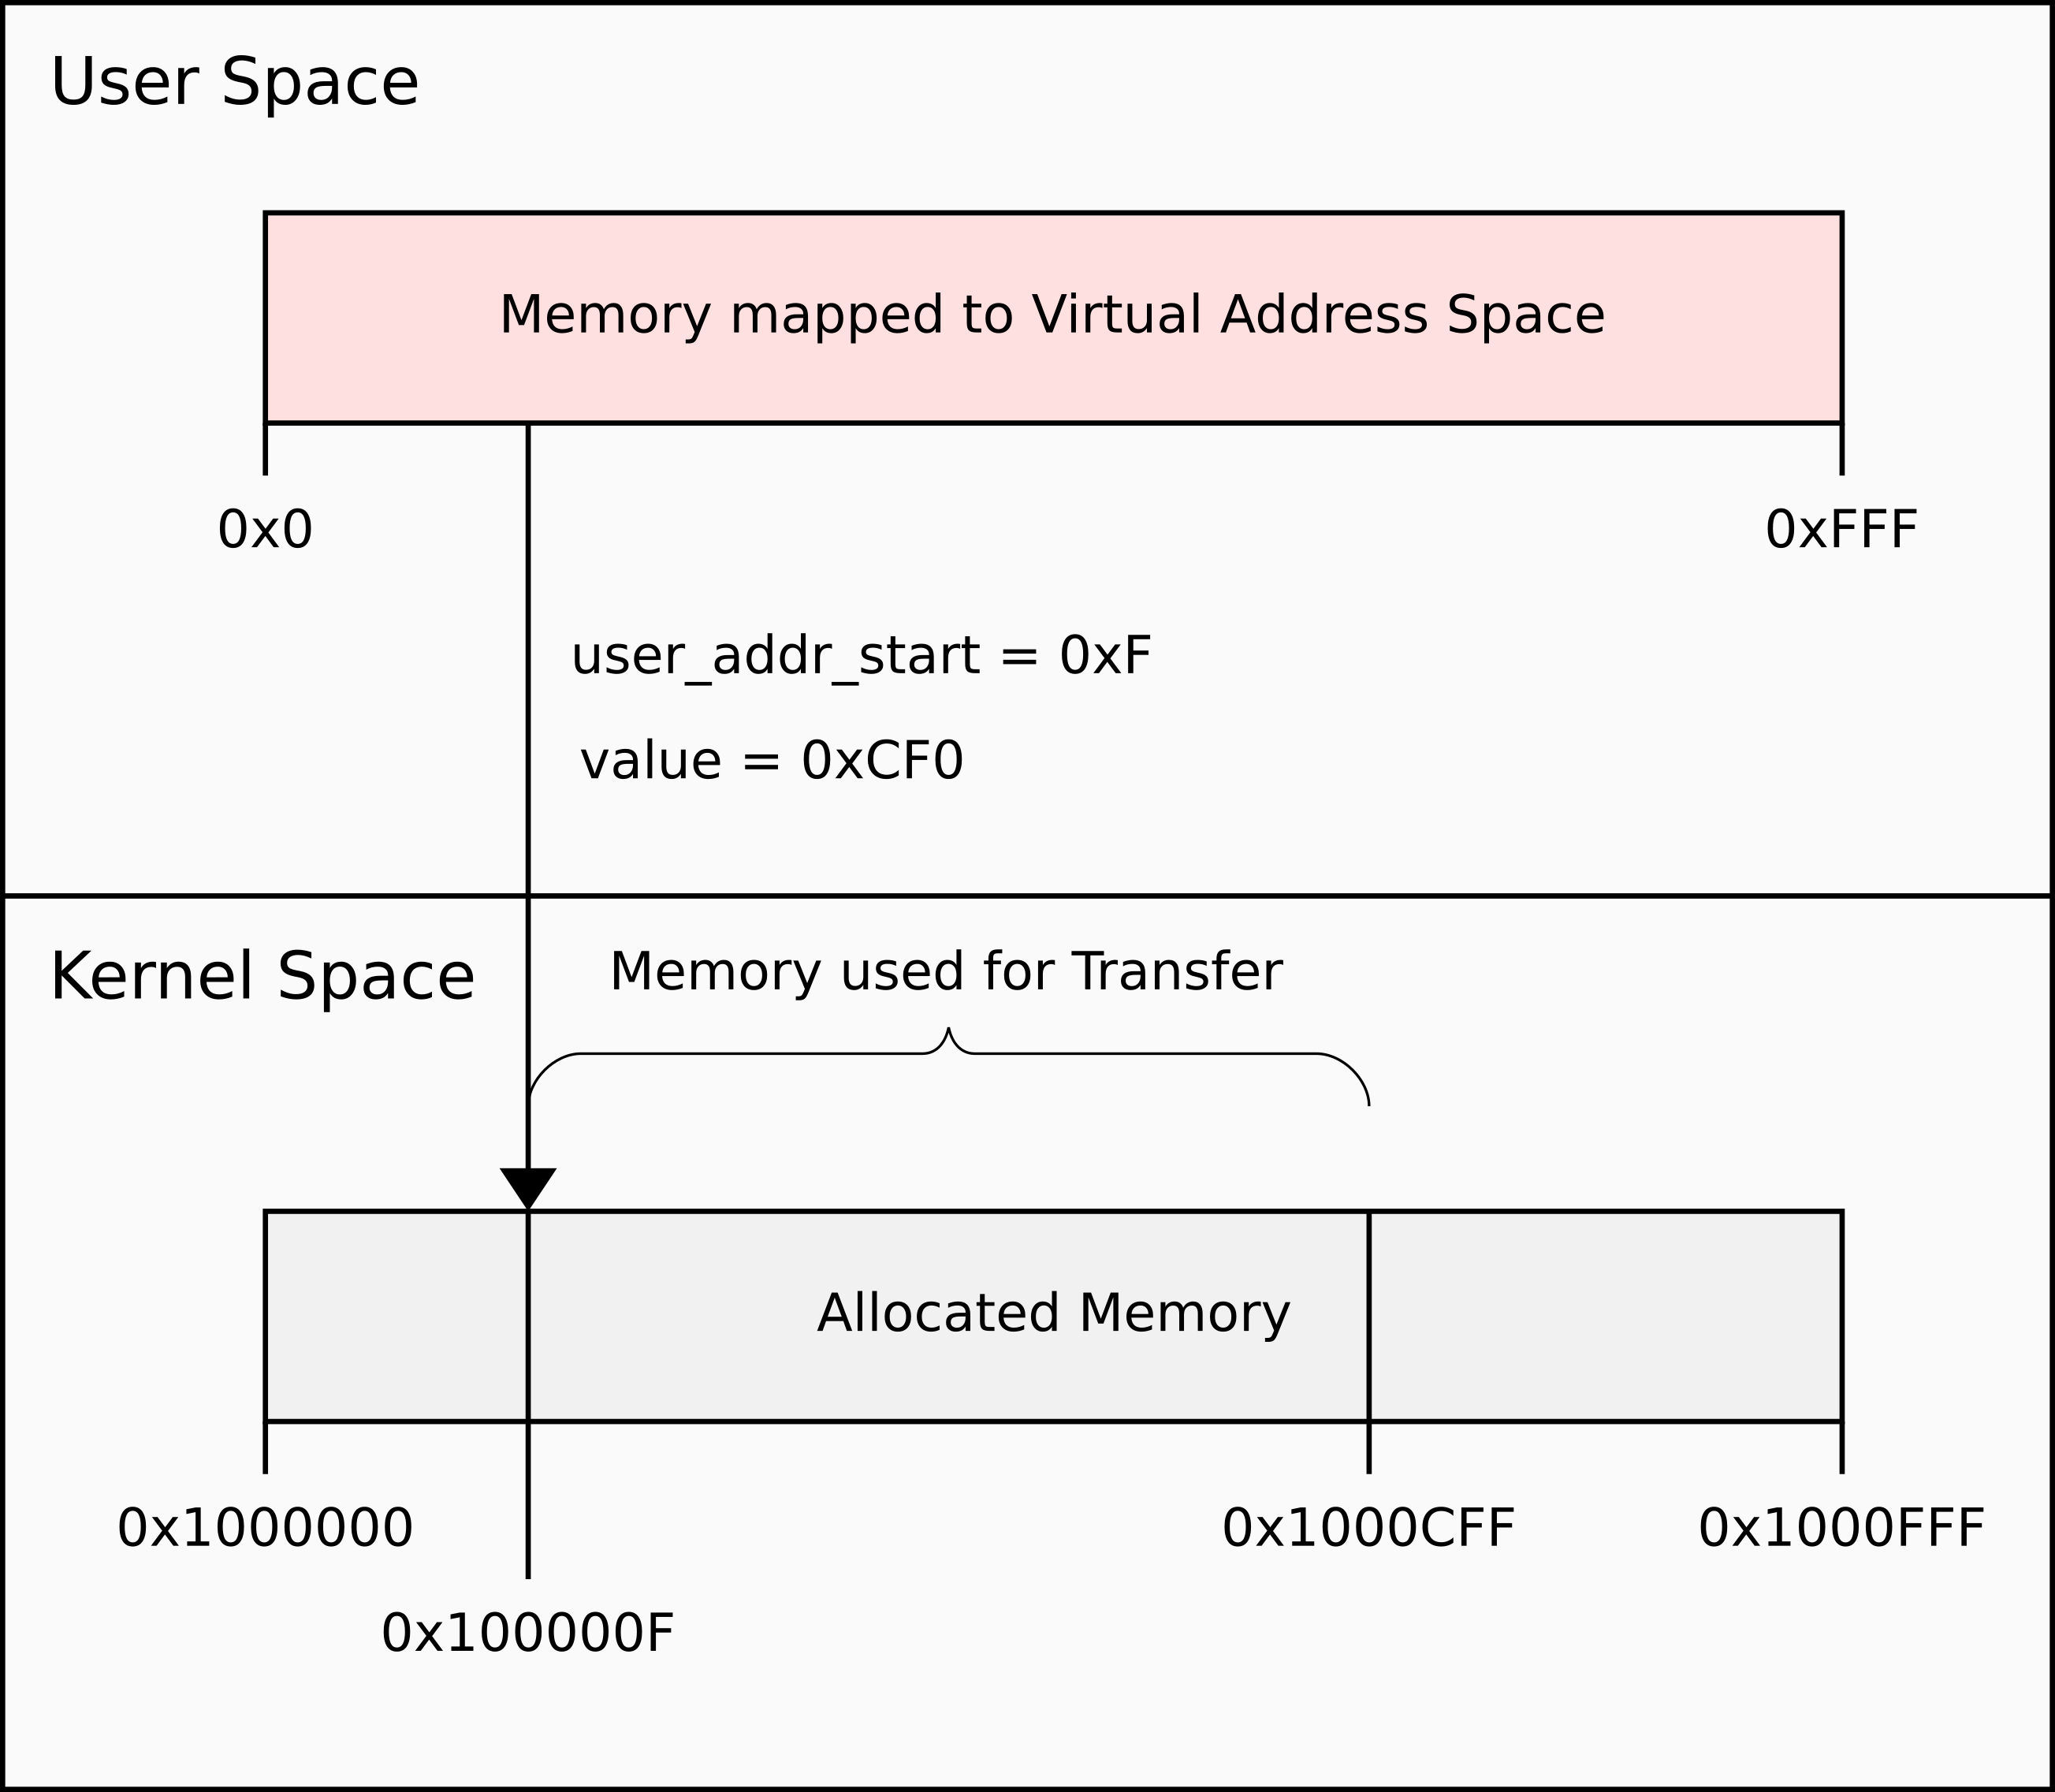
\includegraphics[width=0.5\textwidth,height=0.5\textheight,keepaspectratio]{figs/ioctl_mmap.png}
    \caption{Determining memory area for data transfer.}
    \label{fig:ioctl_mapping}
\end{figure}

After successfully determining the physical address area for the data transfer and acquiring the corresponding memory module, the device driver configures the memory module accordingly.
This is task is accomplished by using the interface functions of the \texttt{as\_reader\_writer} driver, which, in turn, uses the \texttt{as\_regio} device for accessing the hardware registers.
Thereby, the \textit{size} and the \textit{start address} of the \textit{section} is written to the hardware register.
For the remaining parameters, the default values specified in the \texttt{as\_reader\_writer} module driver are used.
As of the \texttt{as\_memwriter}, the \texttt{enable} and \texttt{disable\_on\_no\_go} flags are set.
This prevents the \texttt{as\_memwriter} to store any additional data in its \textit{Fifo Buffer} and thus negatively impacting other parts of the processing chain.
Subsequently, regardless of the memory module being used, the \texttt{go} flag is set to start the operation of the module.

Since the memory module is occupied with a data transfer at this point, it cannot be released by the \texttt{unlocked\_ioctl} method immediately, as the \texttt{as\_memio} device performs a reset on the memory module upon \texttt{open}.
This would terminate the current data transfer and thus has to be prevented.
Therefore, the status flag \texttt{done} is checked for determining whether the memory module has already finished its operation.
Depending on the image processing chain, this may take quite some time, which makes having to actively wait on the operation to finish undesirable.
For this reason, the \texttt{as\_memio} device utilizes a \textit{wait queue}, which is initialized upon creating the \texttt{as\_memio} device.
After checking the \texttt{done} flag, the process executing the \texttt{unlocked\_ioctl} method blocks by calling \texttt{wake\_event\_interruptible}.
If the process is woken up by the \textit{interrupt handler}, it checks the flag again.
In case the flag is still not set, the procedure is repeated.
Otherwise, the \texttt{busy} flag of the utilized \texttt{as\_mmap} device is unset, thus releasing the memory module.
Due to the aforementioned reason, the \texttt{as\_mmap} device currently does not support the \texttt{O\_NONBLOCK} flag.


\subsection{Control Device}

The \texttt{as\_control} device is used for creating and deleting additional devices at runtime.
It is the only device, which is created upon loading the device driver to the kernel and is always associated with the first \textit{minor number}, i.e. "0".
Similarly, it is the device with the first index within the \textit{device array}.
Since it is only used for managing the other devices of the driver, it only utilizes the mutex \texttt{access\_lock} of its associated \texttt{device\_data\_t} structure, which is also initialized upon loading the device driver.
For obvious reasons, \texttt{as\_control} device cannot delete itself or add additional instances of this device type to the device driver.

The functionality of the \texttt{as\_control} device is covered by the file operation method \texttt{unlocked\_ioctl}, which is the only method within its file operation structure.
As for all devices, \texttt{open} has to be called first, before being able to utilize it, however, no implementation is provided for neither \texttt{open} nor \texttt{close}.
This results in using the default methods provided by the kernel.

The mutex \texttt{access\_lock} is utilized to tackle potential race conditions.
Therefore, it always locks its mutex first, when executing its \texttt{unlocked\_ioctl} method.
Since the \texttt{as\_control} device is the only one being available after having loaded the \asterics device driver, adding further devices is the first task performed by the device and is therefore covered first.
In addition to the pointer to the structure representing the device (filp), \texttt{unlocked\_ioctl} method requires two parameters, namely \texttt{cmd} and \texttt{arg}.
The first parameter is used tell the \textit{as\_control} device whether the call to its method stems from the user or kernel space.
This is represented by providing either \texttt{CALLED\_FROM\_USER} or \texttt{CALLED\_FROM\_KERNEL}, respectively.
Both defines are part of the header file \texttt{as\_linux\_kernel\_if.h}, which is part of the \asterics device driver, but is also included for the application software.
Depending on the origin of the call, the \texttt{arg} parameter has to be handled differently.
For calls from kernel space, the data fields of the parameter can be accessed directly using common assignments.
However, if the call originates from user space, the function \texttt{copy\_from\_user} has to be used for copying the data fields of \texttt{arg} into a local structure of the same type, in order to be able to access them.
Generally, the request for creating or deleting devices is performed from user space, since the applications software determines the required devices for operating with the hardware residing on the FPGA.
Nonetheless, the access from kernel space is also supported, in case a different device driver is used for requesting additional devices.
As of the current state, this is mainly for future developments and applications of \texttt{as\_driver}.

The \texttt{arg} parameter, as already suggested, contains the information required by the \texttt{as\_control} device for creating devices.
In order to retrieve the information in a more convenient manner, a structure is used, which posses a number of fields.
This structure is of the type \texttt{as\_ctrl\_params\_t}, which is part of \texttt{as\_linux\_kernel\_if.h}.

The first field of this structure indicates, whether a new device has to be created, by providing \texttt{CMD\_CREATE\_DEVICE} for it.
If this parameter has been provided, the \texttt{as\_control} device checks, whether there are remaining entries in the \textit{device array} for adding an additional device.
This is done by comparing the global variable \texttt{initialized\_devices}, used for tracking the number of currently present devices, with \texttt{MAX\_DEVICES}, defining the maximal number of supported devices.
Each time a new device is added to the device driver, this variable is incremented.
Conveniently, this can also be used for index within the \textit{device array} for inserting the next device.
If the maximal number of devices has been reached, the \texttt{as\_control} device exits with an error message and return value, pointing out this circumstance.
Otherwise, the structure of the current device is initialized with default values, which mainly consists of setting pointers to NULL.
In the next step, the type of the requested device is determined by evaluating the parameter \texttt{dev\_type} of the \texttt{arg} parameter.
The type has to be one of the supported ones, which are also defined in \texttt{as\_linux\_kernel\_if.h}.
Currently supported devices are the \texttt{as\_regio}, \texttt{as\_i2c}, \texttt{as\_memio} and \texttt{as\_mmap} device.
The appropriate file operation structure is assigned to the \texttt{fops} field of the device structure.
The \texttt{interface\_width} and \texttt{flags}, for specifying the memory bus interface and supported direction for data transfer,  are assigned to fields with the same name of the device structure, respectively.
Subsequently, the \texttt{address\_range\_size} size field is assigned with the field with the same name.
The device is then created by using \texttt{cdev\_init} with the appropriate file operation structure.

For the \texttt{as\_regio} and \texttt{as\_i2c} device, a named memory region is requested.
The fields \texttt{dev\_address} and \texttt{address\_range\_size} of the \texttt{arg} parameter are used for specifying the physical start address and the size of the mapped region.
The address of the mapped region is assigned to the \texttt{baseaddress\_virt} field of the device structure.
The offset between the physical and virtual address is stored in the field \texttt{offset}.
Since the memory region has to have a name, \texttt{as\_iic} and \texttt{as\_regio} are used for the devices, respectively. 
However, as the names for the regions are unique, the device driver currently only supports one instance for each of the two device types.

For \texttt{as\_memio} devices, only the field \texttt{dev\_address} of the \texttt{arg} parameter is assigned to the field  \texttt{hw\_module\_addr}, to associate the memory module.
No further resources have to be allocated, since it is handled in its entirety within the file operation methods of the device.
Since the device is the only one associated with a specific hardware module, the aforementioned field is only used for this device.

Regarding the \texttt{as\_mmap} device, a new \texttt{mmap\_info\_t} structure is allocated for storing the \texttt{address\_range\_size} and the allocated physically concurrent memory, using \textit{\_\_get\_free\_pages}.
The size is used for determining the one for the memory allocation.
The start address of the allocated structure is assigned to the \texttt{mmap} field of the device structure.
Lastly, the \textit{wait queue} \texttt{wait} is initialized for allowing the device to block later on.

After the successful initialization of the device, it is published to the kernel by using \texttt{cdev\_add}.
For the \textit{minor number}, the current value of \texttt{initialized\_devices} is added to the first number, which has been used by the device driver.
In this case, the first \textit{minor number} is 0.
Lastly, the \texttt{initialized\_devices} variable is incremented and the mutex is unlocked again.


In order to prevent having to reload the kernel module of the \asterics device driver for removing devices, the \texttt{CMD\_REMOVE\_DEVICE} has been introduced to the \texttt{as\_control} device.
Since an array of a static size is used for managing the devices, deleting single devices would result in holes within the array, which would require a specific handling to avoid trying to access non-existing devices.
Alternatively, an array with a generic size could be used, where the size is increased or decreased each time a new device is created or deleted, respectively.
This approach would necessitate to allocate and reallocate major parts of the device representation at runtime.
As resources may grow scarce the longer the operation system runs, trying to create new devices are more likely to fail.
Usually, devices are deleted and replaced when the hardware processing chain is replaced.
Often times, the majority of the devices are affected, which is the main reason for having the \texttt{as\_control} device delete all other devices at once.
This is accomplished by looping the \textit{device array} and releasing all previously acquired resources.
The variable \texttt{initialized\_devices} is used as the upper boundary of the loop, since it represents the number of devices, which are currently used.
After the \texttt{as\_control} device has finished its task, \texttt{initialized\_devices} is set to 1 again, as only one device is present at this time, i.e. the \texttt{as\_control} device itself.

When deleting devices, care has to be taken, that none of these devices is currently used to prevent undesired behavior.
For this reason, it is recommended to call \texttt{close} on all devices except the \texttt{as\_control} device.


Figure~\ref{fig:control-dev} summarizes the essential functionality and the required steps of the \texttt{as\_control} device.

\begin{figure}[ht]
    \centering
    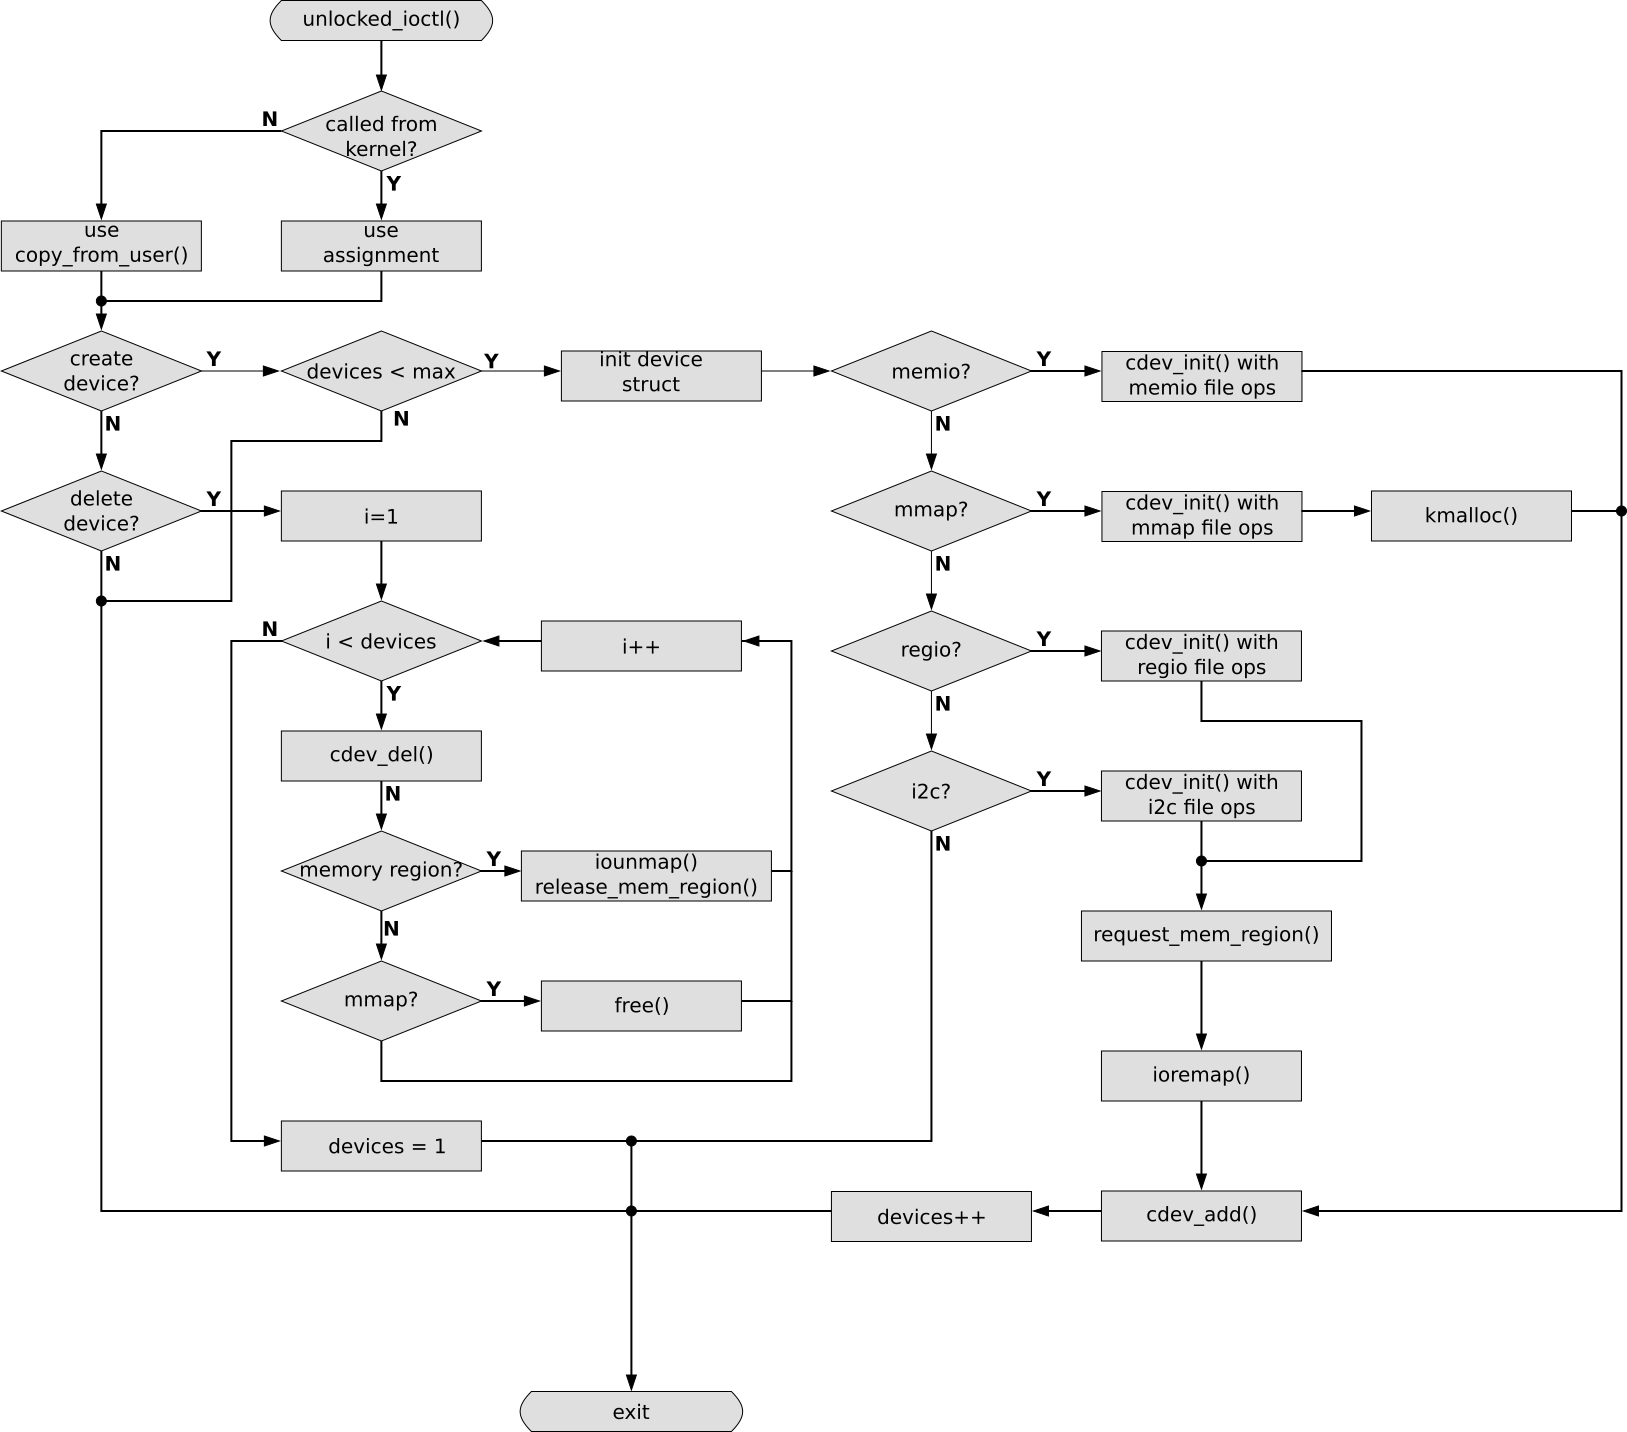
\includegraphics[width=\textwidth,height=\textheight,keepaspectratio]{figs/control_dev.png}
    \caption{Flow chart of the unlocked\_ioctl file operation for the control device}
    \label{fig:control-dev}
\end{figure}


\subsection{Interrupts}
\label{device_driver:interrupts}

\subsubsection{Kernel Timer}

For introducing interrupts to the \texttt{as\_driver}, a global timer has been added for periodically generating interrupt events. 
The timer \texttt{interrupt\_timer} is of the type \texttt{struct timer\_list}, which is part of the timer API of the kernel. 
The timer uses jiffies for determining its interval between interrupt events. 
For the Zynq platform, the default setting of the system uses the value 100 for its HZ definition (param.h which is part of the system). 
This results in a granularity for the timer interval of 10 ms. 
The timer is initialized upon loading the device driver into the kernel, where the parameter \texttt{TIMER\_INTERVAL} is used for the actual interval of the timer. 
For its interrupt handler, the timer is associated with the function \texttt{timer\_callback}, which is called when the timer expires, i.e. after the configured interval. 
The timer is triggered for the first time at the end of the initialization of the device driver and registers itself within its interrupt routine. 
In order to prevent race conditions when the device driver is unloaded, the flag \texttt{timer\_shutdown} is used. This flag is set exit method of the device driver before trying to delete the timer. 
The timer checks this flag before trying to register itself to run again. 
If this flag is set, the timer does not run again.

As aforementioned, the main purpose of the interrupt handler is to manage blocking \texttt{as\_memio} and \texttt{as\_mmap} devices. 
Since interrupt routines have to be executed in a timely manner, the amount of operations of it are rather limited. As \texttt{as\_driver} may utilize several devices, serving them can be time consuming task and is therefore not suited to be performed within the interrupt handler itself.
For this reason, the shared work queue by the kernel is used, into which the work item \texttt{timer\_wq}, is inserted. 
This work item is associated with a function, which is executed when the work item is scheduled to run by the work queue. 
The function in turn is used for carrying out the actual operations required for handling the \texttt{as\_memio} and \texttt{as\_mmap} devices. 
The work item is set up and associated with the function \texttt{data\_transfer\_update\_task} by calling the macro \texttt{INIT\_WORK}. 
The function is then scheduled by the \texttt{timer\_callback} function of the timer.
This allows the interrupt handler of the timer to return in a timely manner, since the only two operations performed by it is calling \texttt{schedule\_work} for the inserting the work item into the queue and registering itself to run again. 
The initialization of the work item is done just before configuring the timer, in order to be used.

The first part of the \texttt{data\_transfer\_update\_task} function handles any \texttt{as\_memio} devices, which are currently in use. 
In a first step, the function iterates all currently initialized devices within the \textit{device array} to find \texttt{as\_memio} devices. 
This is determined by examining the \texttt{fops} field of the device structure, whether it points to the file operation structure used for the \texttt{as\_memio} device. 
If this is the case, it checks if the \texttt{memio\_active} flag is set, which means the user has called open on the corresponding device. 
Subsequently, the \texttt{register\_intr} flag has been set, if the device is currently sleeping. 
The \texttt{data\_transfer\_update\_task} sets the condition variable \texttt{wake\_up\_cond} and calls \texttt{wake\_up\_interruptible} on the device, which causes it to wake up and check if new data has become available. 
For \texttt{as\_memio} devices which are in use but the \texttt{register\_intr} flag has not been set, the function \texttt{as\_memio\_hw\_update} of the \texttt{as\_memio} module driver is called. 
This guarantees, that data in the \textit{Ring Buffer} is not "stuck" for an extended period of time, before being transferred. 
Otherwise the user may wait indefinitely for the data to actually appear on memory or at the processing chain on the FPGA.
For the \texttt{as\_mmap} devices, the \texttt{fops} field is also checked for determining the device. 
This is performed at the same time as for the \texttt{as\_memio} devices, to prevent having to loop the devices twice. 
Similar to the \texttt{as\_memio} device, the \texttt{register\_intr} flag is examined before setting the \texttt{wake\_up\_cond} variable and calling \texttt{wake\_up\_interruptible} on the \texttt{as\_mmap} device.

\subsubsection{Hardware Module}
%TBD ?!

\construction{section}


\subsection{Driver Initialization and Deinitialization}
Once \texttt{as\_driver} has been successfully compiled, it can be loaded as a kernel module.
The device driver requests a single major number and the configured amount of minor numbers, starting with 0.
The major number is used to tell the kernel which driver is associated with a given device.
Since a device driver may be responsible for more than one device, as is the case for the \asterics device driver, the minor number is used to distinguish between the devices.
Currently, the device driver is assigned a major number dynamically by the operating system, instead of having it request a specific number itself.
This prevents potential conflicts with other drivers, if the requested major number is already in use or a different driver tries to request the same major number at a later point.
After the major number and minor numbers have been acquired, a device class is created for grouping the devices.\newline

Since the devices depend on a specific \asterics-chain, they have to be created dynamically by the \texttt{as\_control} device.
For this reason, the device driver creates the \texttt{as\_control} device upon initialization and assigns the first minor number (0) to it.
The \texttt{as\_control} device is created, by initializing the first device in the device list as the \texttt{as\_control} device.
Additionally, the number of initialized devices is incremented by one.
However, the device driver does not create a device node on the file system itself, in order for the user to choose the name and location on his own.
Rather, the user is expected to create the device node to the actual device.

Lastly, the interrupt timer is set up by mapping its service routine and configuring the time interval, at which the service routine is to be executed.
The time interval can be configured as part of the compile-time options of \texttt{as\_driver}.

As for unloading the \asterics device driver, the \texttt{timer\_shutdown} flag is set to prevent the interrupt timer to run again before deleting it using \texttt{del\_timer\_sync}.
Subsequently, all currently initialized devices, except for the \texttt{as\_control} device, are deleted by releasing all resources to the operating system and removing any memory mappings, first.
After this step, the device driver requests the kernel to delete the devices with their corresponding minor number.
Once their is no device remaining, the \texttt{control} device is deleted in the same way, before the \textit{device class} is destroyed and the driver itself is unregistered.
The major number and all minor numbers are released and may be assigned to a different driver.


\subsection{Application Notes}

\subsubsection{Building the Kernel Module}
There are two options for building the Linux kernel module, either using a cross-compiler on the host platform or the native compiler on the target platform itself.
Both require the proper \textit{kernel headers} to be installed (usually at "/lib/modules") for building Linux kernel modules for the target architecture.
A \texttt{Makefile} is provided for the \texttt{as\_driver} with options for building the Linux kernel module on either the host or the target.
Comments within the \texttt{Makefile} describe how either one can be used.
The option for compiling on the host platform, however, has only been tested for Xilinx platforms so far.
Xilinx ships ships its own libraries and tools, such as the compiler.
Additional steps may be required for other vendors but should work in the same manner, by simply referring to the path where the kernel headers have been installed.

More information for installing the kernel headers are provided at the \href{http://ti-wiki.informatik.hs-augsburg.de/doku.php?id=linux_microzed}{\textit{Technical Wiki}}.

\subsubsection{Creating Devices}
Except for \texttt{as\_control}, all devices have to be created within \texttt{as\_driver} since they depend on the actual \asterics-chain.
Devices are defined within \texttt{as\_hardware.c}, which provides interfaces for obtaining the number and list of devices.
The source file \texttt{create-devices.c} shows the required steps for creating and deleting devices using the interfaces of \texttt{as\_hardware.c(/h)}.
This file can be found at "tools/as-linux/src/kernel\_module/create-devices"
The shell script files \texttt{load\_devices.sh} and \texttt{unload\_devices.sh} use the executable of \texttt{create-devices.c}.

The whole directory ("create-devices") can be copied into the one of the system for using the system specific \texttt{as\_hardware.h/c}.

\subsubsection{Creating Device Nodes}

In order to use the devices of the \asterics driver, corresponding device nodes have to be created on the file system.
The \textit{minor} numbers are assigned in the same order as the devices are created, starting with "1" ("0" is the \texttt{as\_control} device).
However, the \textit{major} number of the kernel module has to be looked up, since it is dynamically assigned by the Linux kernel.
This can be achieved by searching for \texttt{as\_driver} in "/proc/devices".
The actual device node is then created with \textit{mknod}.

The two shell scripts \texttt{load\_devices.sh} and \texttt{unload\_devices.sh} are provided for creating and deleting device nodes.
The \textit{minor} numbers of the device nodes have to match the devices listed in \texttt{as\_hardware.c}.
 

